\chapter{Related work}
\label{Related work}

In this chapter, we overview common approaches to solve problems with point clouds. We review common techniques, models, and algorithms for point clouds.

In Section~\ref{Deep learning approaches for point cloud} and Section~\ref{Point-based Methods} we review common approaches on how to use point clouds in deep learning, along with preprocessing methods for 3D point data.

In Section~\ref{Human pose estimation} we review models and techniques for the task of human pose estimation, both for 2D and 3D spaces.

In Section~\ref{Capsule network} we review the initial work on the capsule network which were released for the task of image classification. Also, we review few works which adapt capsule networks for 3D point cloud data.

\section{Deep learning approaches for point cloud}
\label{Deep learning approaches for point cloud}
The different number of points and high dimensionality of the point cloud input makes it challenging to use regular 2D convolutions. The typical approach for such an issue is the conversation of the point cloud to a different format. Such approaches are projection-based methods, volumetric-based methods, and other geometric-based methods.
\subsection{Projection-based methods} 
Projection-based methods take point cloud and project it into a different panel view. After the projection, each view provides a set of combined features for target classification, regression, or segmentation. The critical challenge for the projection-based algorithm is the multi-view feature aggregation into one global feature space.

MVCNN \parencite{su_multi-view_2015} is the first CNN-based architecture which recognize rendered views of different shapes independently from each other. The model's performance shows that even from one view the 3D shape could be recognized with competitive accuracy. Adding more views increase the overall accuracy of the model. The processing pipeline if the MVCNN is shown in Figure~\ref{img:mvcnn}.

\begin{figure}[htbp]
    \centerline{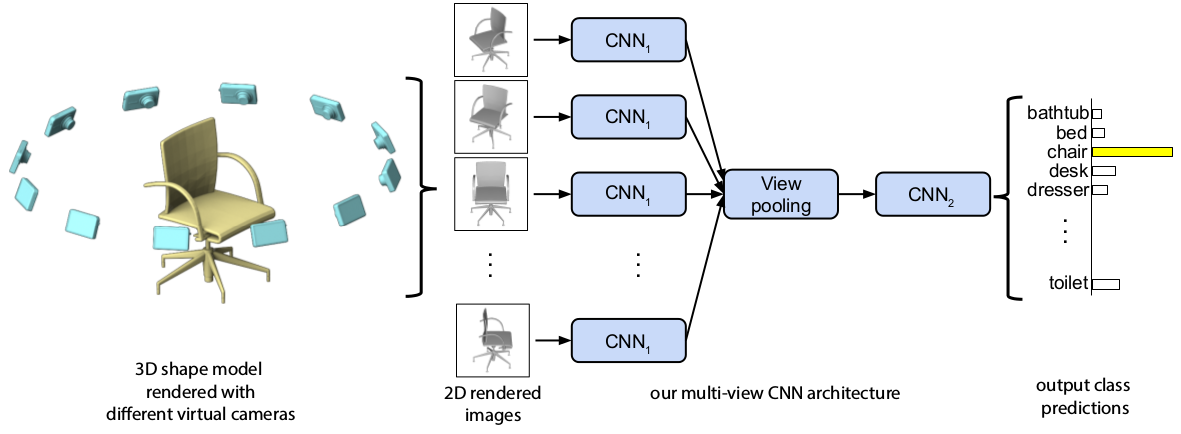
\includegraphics[scale=0.4]{Figures/mvcnn.png}}
    \caption{MVCNN processing pipeline  \parencite{su_multi-view_2015}}
    \label{img:mvcnn}
\end{figure}


MHBN \parencite{yu_multi-view_2018} (Multi-view Harmonized Bilinear Network) is the continuation of MVCNN. The approach proposes to integrates local convolutional features by harmonized bilinear pooling to produce a compact global descriptor.
To persist the information from different views, the View-GCN \parencite{wei_view-gcn_2020} proposes constructing view-graph with multiple views as graph nodes, then designing a graph convolutional neural network over view-graph to learn discriminative shape descriptor hierarchically.
All projection-based methods struggle from high memory consumption and high computational complexity since, for one feature extraction, the model should be run for the number of different views.

\subsection{Volumetric-based methods} 
Volumetric-based methods map the point cloud into a 3D grid. Then conventional 3D convolutions are using for feature extraction.
VoxNet \parencite{maturana_voxnet_2015} is the first method that exploits the volumetric representation of the point cloud. In this work, each cloud point is mapped to a discrete voxel point. The size of the target grid is 32 x 32 x 32 voxels. After the mapping, three convolutional layers are using to produce the target feature representations. Processing steps of VoxNet is shown in Figure~\ref{img:voxnet}

\begin{figure}[htbp]
    \centerline{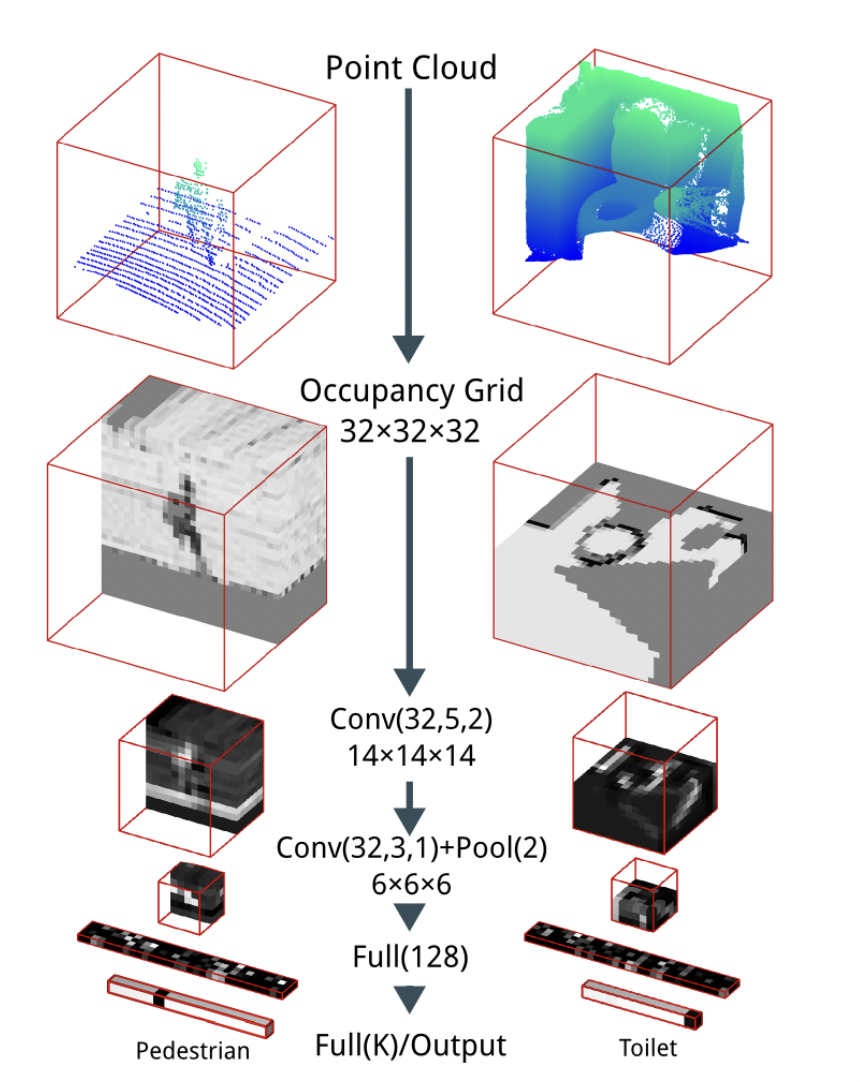
\includegraphics[scale=0.4]{Figures/VoxNet.png}}
    \caption{VoxNet processing pipeline  \parencite{maturana_voxnet_2015}}
    \label{img:voxnet}
\end{figure}

The more advanced volumetric-based models use octrees data structure. OctNet \parencite{riegler_octnet_2017} propose to represent the point cloud as several octrees along a regular grid (Figure~\ref{img:octTree}), each octree is encoded as a bit string, and features are generated through naive arithmetic. This approach reduces the memory consumption of the model during the training and inference stages.
The next iteration of octrees representation of point cloud is proposed in O-CNN \parencite{wang_o-cnn_2017}. The model uses 3D convolutions to extract features from octrees. This model also uses octree representation. The model takes the average normal vectors if 3D model from leafs of octants and runs 3D CNN on this to perform classification.

\begin{figure}[htbp]
    \centerline{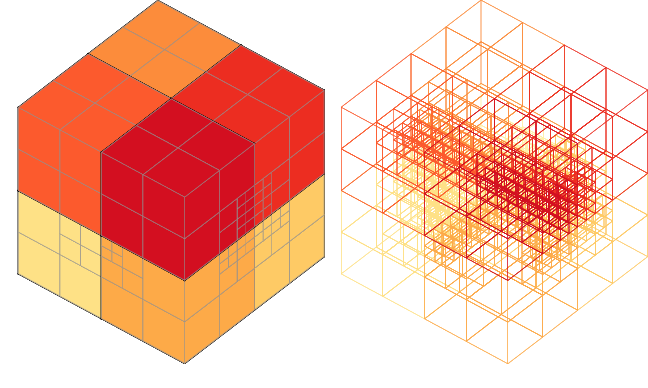
\includegraphics[scale=0.4]{Figures/OctNet.png}}
    \caption{An example of octree grid \parencite{riegler_octnet_2017}}
    \label{img:octTree}
\end{figure}

\section{Point-based Methods}
\label{Point-based Methods}
Compared with projection-based methods and volumetric-based methods that aggregate points from a spatial neighborhood, point-based methods attempt to learn features from individual points. Most of the recent work focuses on this direction.

The first work which uses a point-based approach is PointNet \parencite{qi_pointnet_2017}. PointNet learns pointwise features independently with several MLP layers and extracts global features with a max-pooling layer. The input (an $n \times 3$ 2D tensor) is first multiplied by an affine transformation matrix predicted by a mini-network (T-Net) to hold invariance under geometric transformations. The point set is then passed through a group of MLPs followed by another joint alignment network, and a max-pooling layer to obtain the final global feature. The model's architecture is depict in Figure~\ref{img:pointnet}

\begin{figure}[htbp]
    \centerline{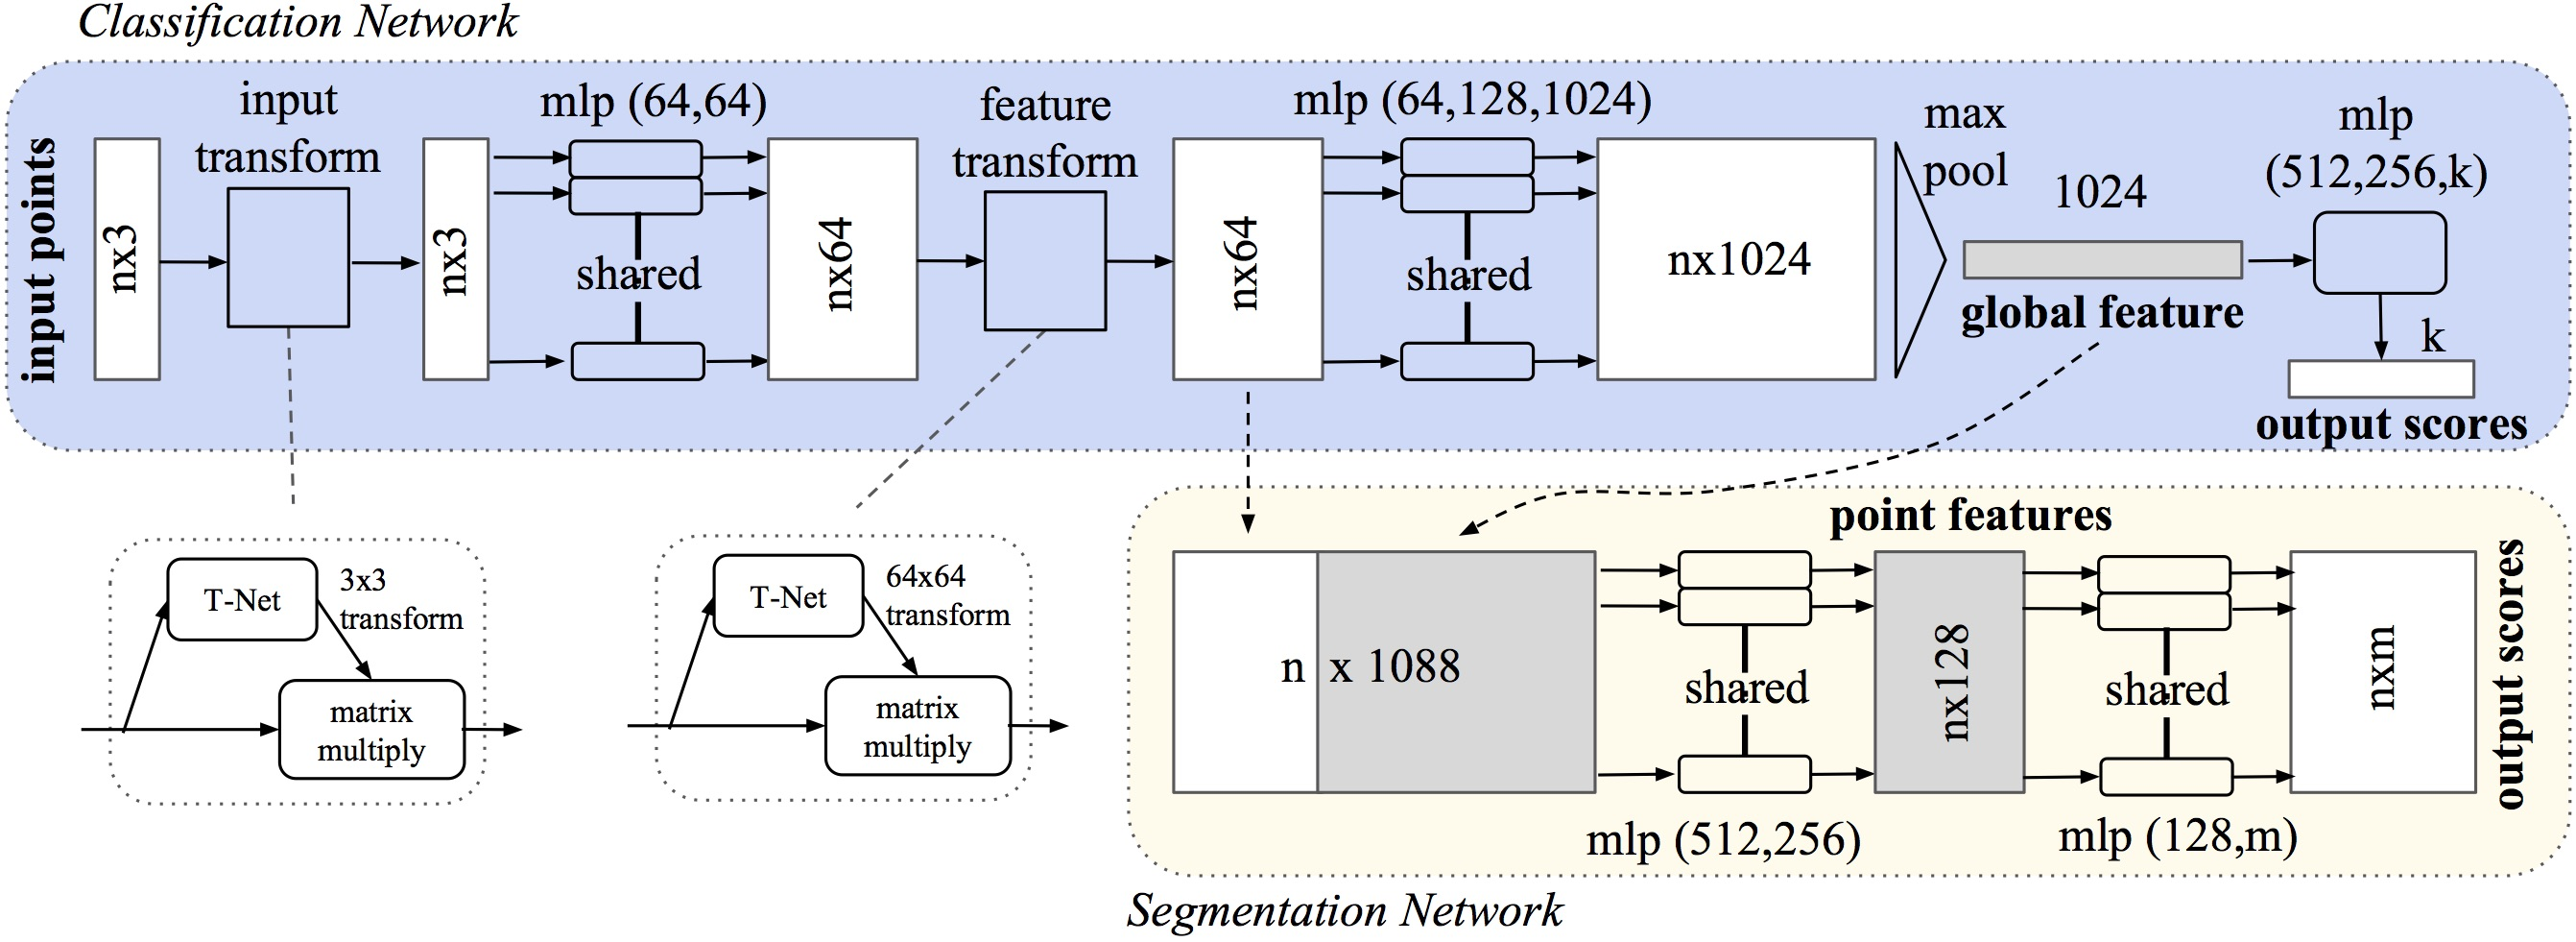
\includegraphics[scale=0.15]{Figures/pointnet.jpeg}}
    \caption{PointNet architecture \parencite{qi_pointnet_2017}}
    \label{img:pointnet}
\end{figure}


The second iteration of PointNet is PointNet++ \parencite{qi_pointnet_2017-1}. PointNet++ introduces a hierarchical neural network that applies PointNet recursively on a nested partitioning of the input point set. Using metric space distance, the model could learn local features with increasing contextual scale.
The state-of-the-art model for point-based classification is Point Attention Transformers \parencite{yang_modeling_2019}. The research for the first time proposes the mechanism of sampling which is end-to-end and task agnostic. The sampling is named "Gumbel Subset Sampling" - GSS. This sampling is used to select the most representative subset of the point cloud from the initial data. Using Gumble-Softmax, the model could provide a continuous point subset in the training phase, and a strict discrete subset in the test phase. Using such an approach the model is able to learn a more robust representation of the input data with less computational complexity.

\section{Human pose estimation}
\label{Human pose estimation}
The latest research approaches in the field of human pose estimation are based on deep learning.
There are two main approaches to the task:
\begin{itemize}
  \item pose estimation based on 2D images (mostly RGB);
  \item pose estimation based on the 3D point cloud.
\end{itemize}

The latter approach is more recent and promising. The 3D perspective gives more information for the models about body position in the space. Also, 3D point clouds mitigate the issue with occluded parts of the body. 2D image is a 2D projection of 3D space, and this transformation leads to the loss of information.

\subsection{Image-based methods}
The approaches for 2D image human pose estimation are divided into two types:
\begin{itemize}
  \item top-down approach
  \item bottom-up approach
\end{itemize}
In the top-down approach, the first step is person detection and then pose regression. In the bottom-up approach, all body parts are detected first and then grouped according to the body's position.

OpenPose \parencite{cao_openpose_2019} is the most popular example of bottom-up approaches for multi-person pose estimation. The network first extracts features from the image using the VGG feature extractor. Then features are passed to two separate branches, the first branch predicts body parts key points, the second branch predicts the associativity between body parts. The result of human pose estimation from OpenPose is shown in Figure~\ref{img:openpose}.

\begin{figure}[htbp]
    \centerline{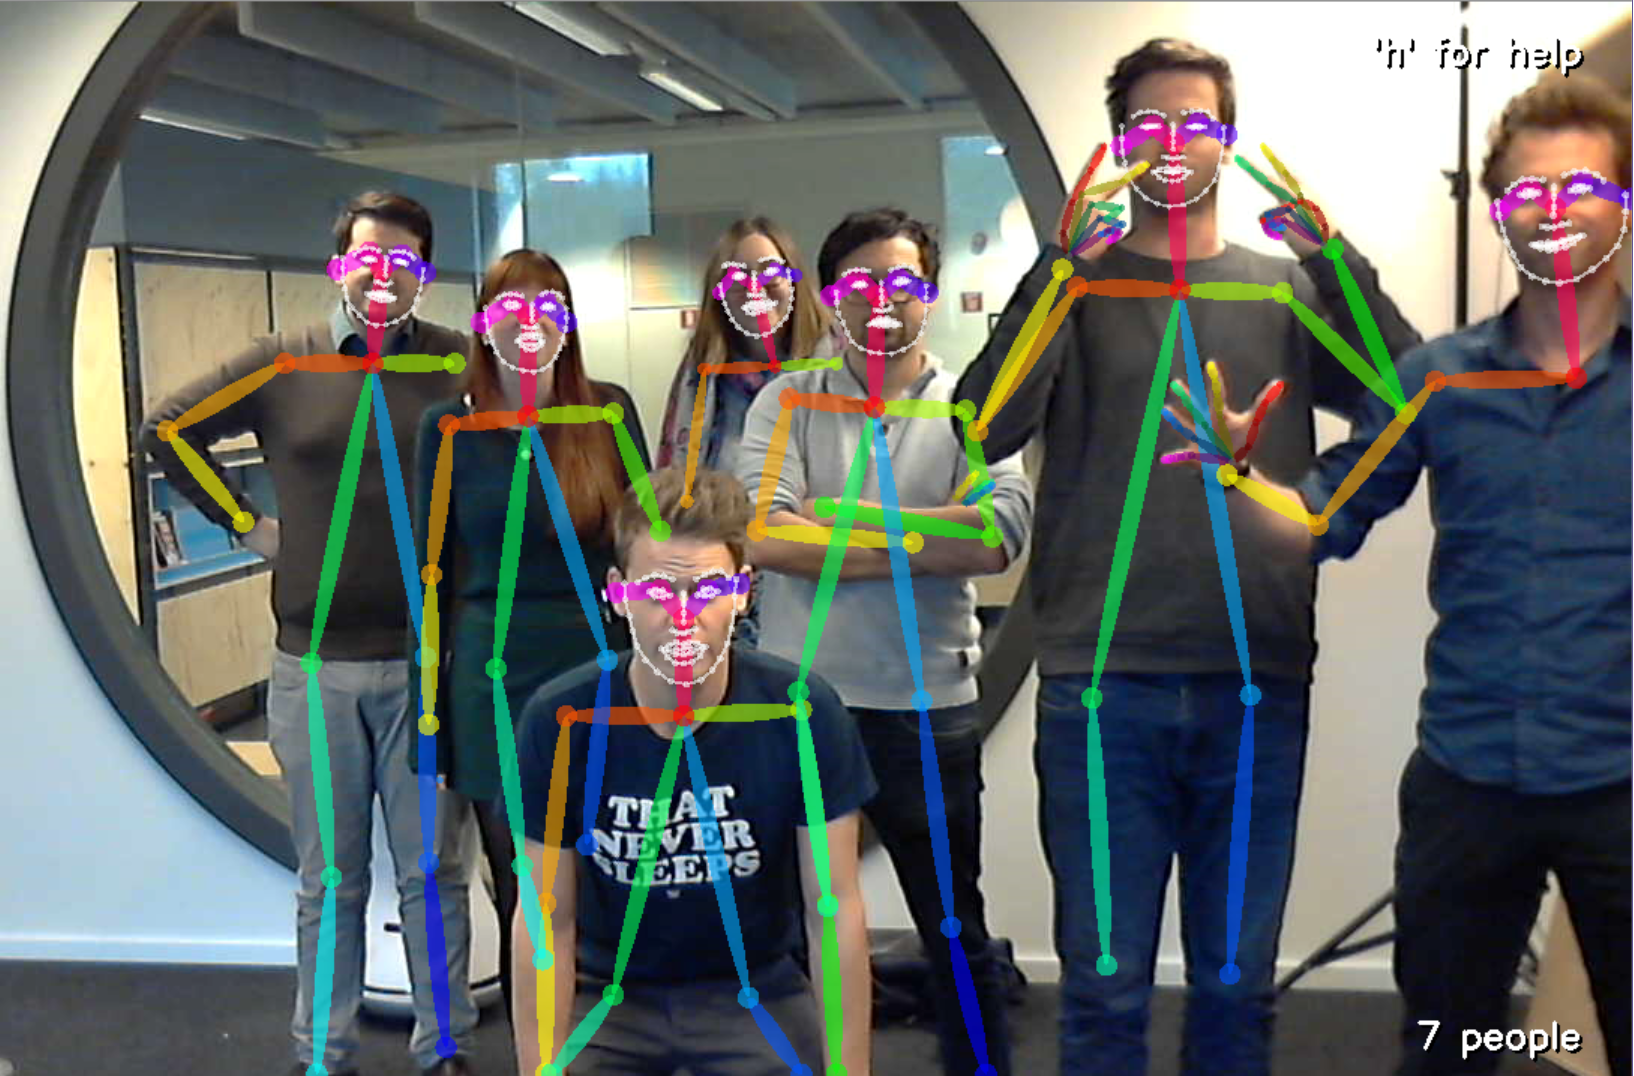
\includegraphics[scale=0.15]{Figures/OpenPose.png}}
    \caption{An example OpenPose network result  \parencite{cao_openpose_2019}}
    \label{img:openpose}
\end{figure}


RMPE (AlphaPose) \parencite{fang_rmpe_2018} is a top-down model.
This approach proposes to use a four-stage pipeline. The first step is Symmetric Spatial Transformer Network (SSTN). In this step, the model extracts the human region using a bounding box. The second step is a Single Person Pose Estimator (SPPE). This step model uses extracted human regions to estimate key joints of the human body. The third step is spatial De-Transformer Network (SDTN). This step remap estimated human joint coordinates back to the original coordinate system. The last step is parametric pose Non-Maximum Suppression (NMS). This step handles the issue with redundant pose deductions.

\subsection{point-cloud-based methods} 
Point cloud-based estimation is a relatively young field due to the recent growth of popularity of point cloud scanning devices.

The first model for human pose estimation based on point cloud was presented by \cite{diaz_barros_real-time_2015}. The paper presents an approach where based on a predefined human body skeleton the input point cloud is clustered using PCA and Expectation maximization algorithms.

The recent work in this field is presented by \cite{zhou_learning_2020}. The work takes point clouds as input data and model the surface of the object, in this research - human body, using deep human pose network. The pros of this approach is that it's an end-to-end model. It takes 2D depth image, transforms it to 3D point cloud, and then estimate key human joint coordinates. The model's architecture is shown in Figure~\ref{img:humreg}

\begin{figure}[htbp]
    \centerline{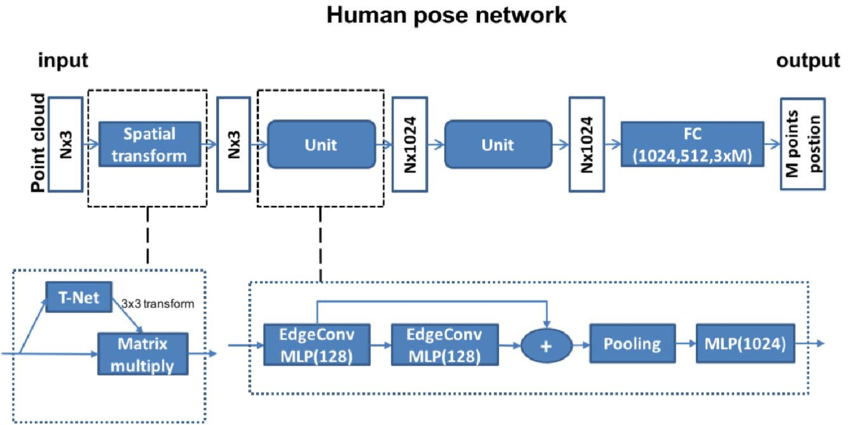
\includegraphics[scale=0.4]{Figures/human-regression-network.png}}
    \caption{Architecture of DNN presented by \parencite{zhou_learning_2020}}
    \label{img:humreg}
\end{figure}

More point cloud human pose estimation methods will be covered in the next subsection. The next subsection covers models which are based on capsule architecture.

\section{Capsule network}
\label{Capsule network}
The concept of the capsule was first proposed by Hinton \parencite{sabour_dynamic_2017} and has been widely used in 2D and 3D deep learning \parencite{kakillioglu_3d_2020, qin_detecting_2020, duarte_videocapsulenet_2018, lalonde_capsules_2018}.

Capsules are represented as a set of vectors. The length of the capsule's vector represents the probability of the object's presence. The direction of the vector describes the object's property e.g. position, viewpoint, size, shape, etc. For capsules' training Hinton proposes a new algorithm \parencite{sabour_dynamic_2017} called dynamic routing. The forward pass with dynamic routing propagates the input data from lower-level capsules to higher-level ones. Lower-level capsules pass learned and predicted data to the higher-level capsules. If multiple lower-level capsules agree (activated) then higher-level capsules activate accordingly. With each iteration of dynamic routing, each capsule gets more accurate.

\subsection{Capsule networks for point cloud classification}
The first work where capsule networks were applied to the problem of point cloud classification is 3DCapsNet \parencite{cheraghian_3dcapsule_2018}. In this work, a new capsule-based layer is proposed - ComposeCaps. ComposeCaps learns spatially relevant feature mapping that can be exploited for 3D point cloud classification. The architecture of the network is shown in Figure~\ref{img:3DCapsNet}

\begin{figure}[htbp]
    \centerline{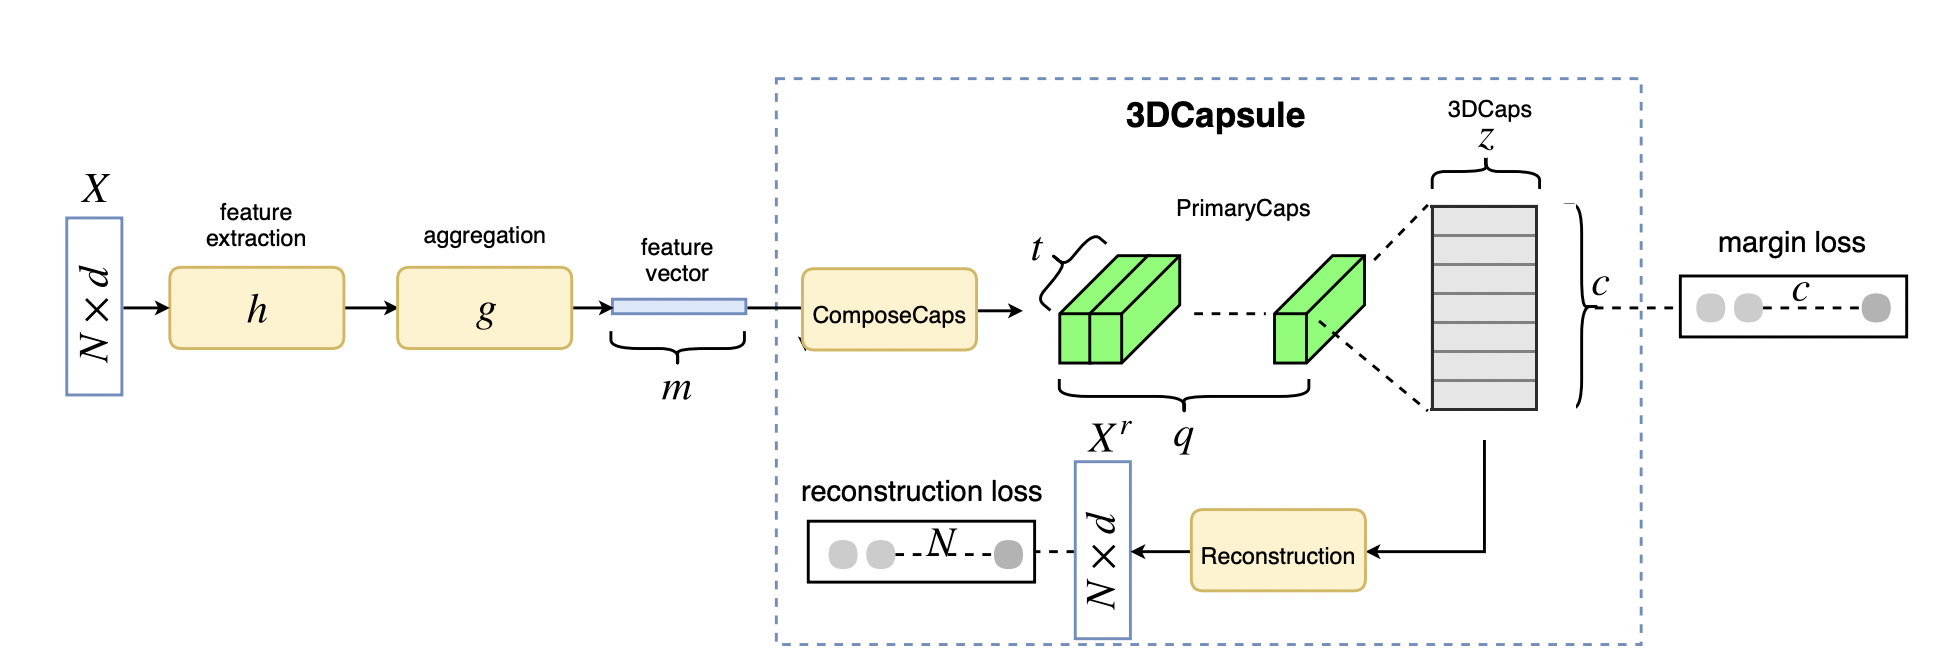
\includegraphics[scale=0.4]{Figures/3DCapsNet.png}}
    \caption{The architecture of 3DCapsNet \parencite{cheraghian_3dcapsule_2018}}
    \label{img:3DCapsNet}
\end{figure}

The second iteration of capsule applicability to 3D classification is the 3D point capsule network \parencite{zhao_3d_2019}. 3D point capsule network is an auto-encoder designed based on capsule networks. In this work researchers propose new architecture with a capsule network encoder that encodes input point cloud to capsules' latent space, and a decoder that decodes latent capsules. The proposed architecture works for several common point cloud-related tasks, such as object classification, object reconstruction, and part segmentation.

\subsection{Capsule networks for point cloud regression} 
The only work which is currently presented on the topic of point cloud regression is Capsule-HandsNet \parencite{wu_3d_2020}. This project is inspired by this research. Capsule-HandsNet uses model based on capsule auto-encoder proposed in \cite{zhao_3d_2019}. The model is an end-to-end, it takes hand point cloud and predicts key joints. The latent space of the model provides an ability to "memorize" the internal structures of the object such as symmetry, junction, relative location of object's parts, etc. The restored point cloud is combined from local patches predicted by capsules inside of the decoder (Figure~\ref{img:capshandnet}).   

\begin{figure}[htbp]
    \centerline{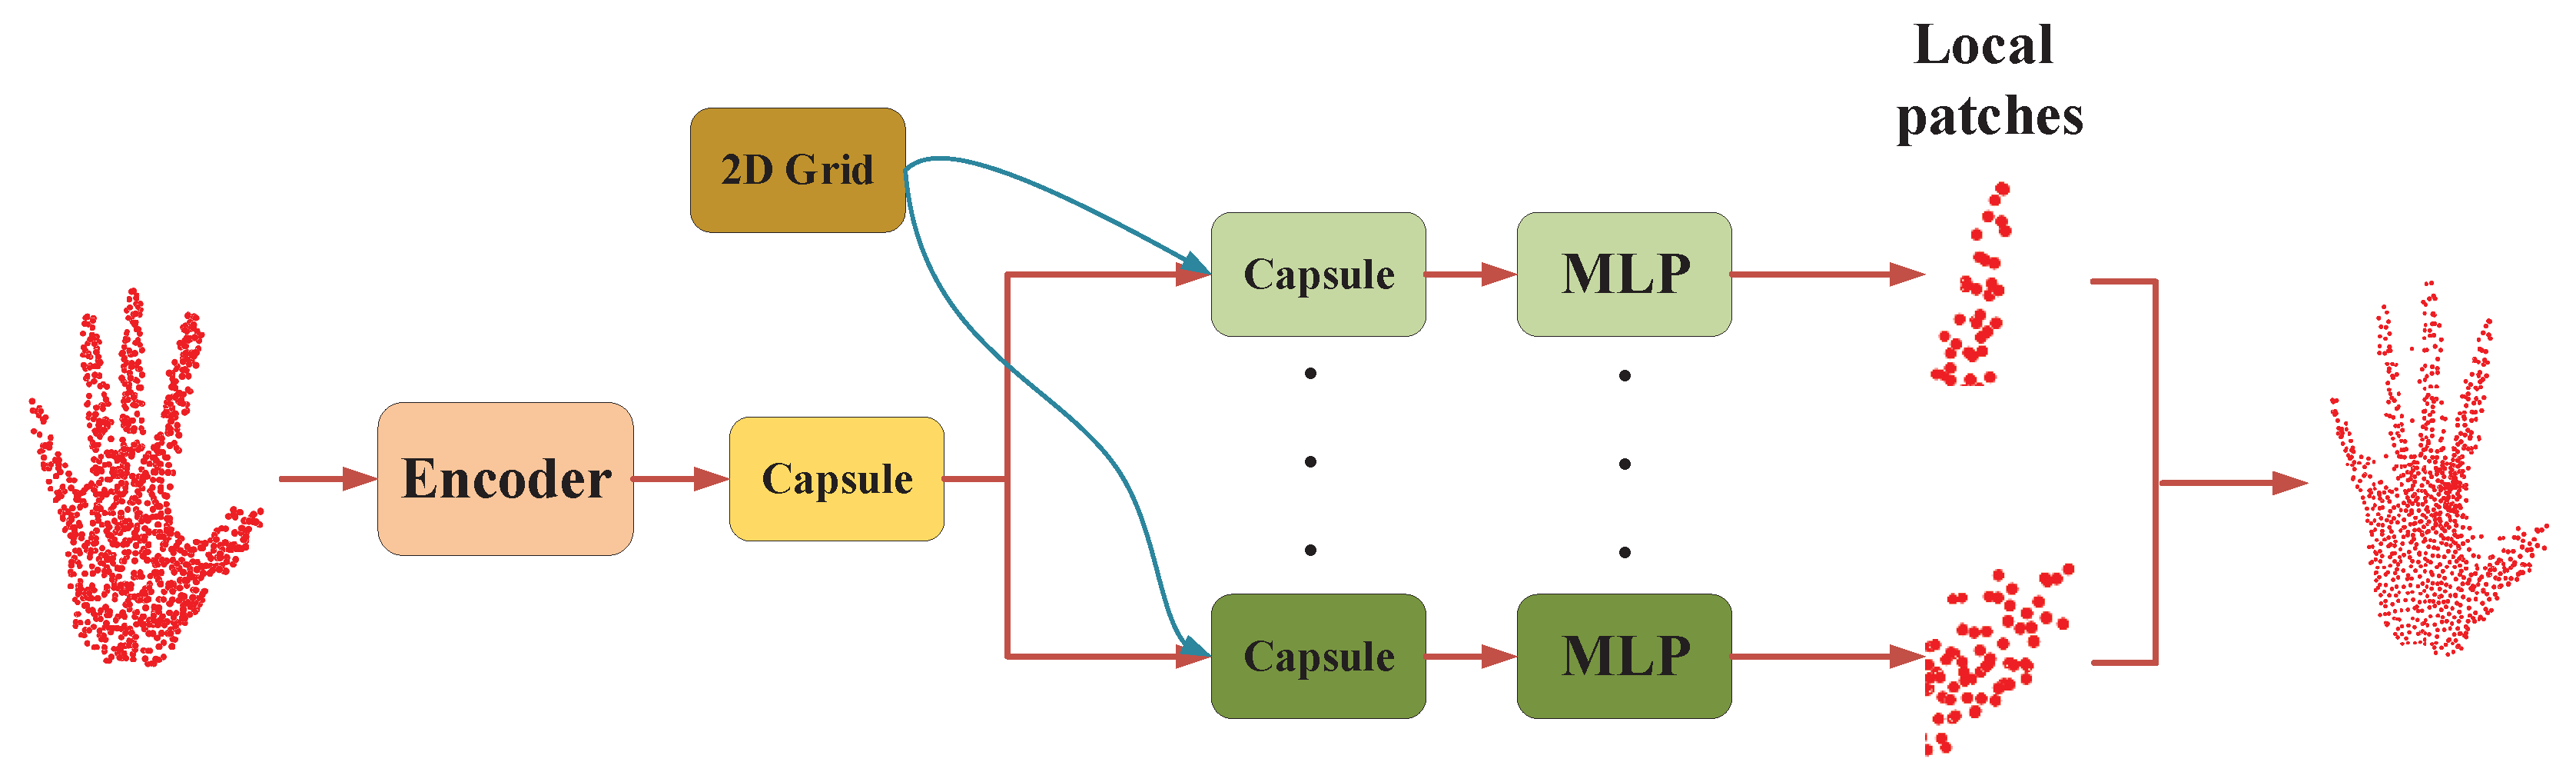
\includegraphics[scale=0.9]{Figures/caps-hand-net.png}}
    \caption{Reconstructed point cloud from capsule local patches \parencite{wu_3d_2020}}
    \label{img:capshandnet}
\end{figure}
